\documentclass{article}
\usepackage{graphicx} % Required for inserting images
\usepackage {tikz}
\usepackage{url}
\usetikzlibrary {shapes, arrows, positioning}

\begin{document}

\section*{}

\section{MM22B046}
\subsection{Details}

\begin{itemize}
  \item Pranav Sridhar
  \item MM22B046
  \item MentalLink
\end{itemize}
\subsection{Equation}

\begin{equation}
P(X_{t+1}=s_{t+1}|X_{t}=s_{t},X_{t-1}=s_{t-1},\ldots ,X_{0}=s_{0})=P(X_{t+1}=s_{t+1}|X_{t}=s_{t})
\end{equation}

\subsection{Description}
Markov chains are mathematical models used to study the behavior of systems that undergo a sequence of random events or transitions. They are named after the Russian mathematician Andrey Markov, who pioneered their study in the early 20th century.
In a Markov chain, the future state of the system depends only on its current state and is independent of its past states. This is known as the Markov property or the memoryless property. The system can transition from one state to another according to certain probabilities associated with each possible transition.
Formally, a Markov chain is defined by a set of states and a transition matrix. The transition matrix represents the probabilities of moving from one state to another. Each row of the matrix corresponds to a current state, and the elements in that row represent the probabilities of transitioning to each possible next state.

Markov chains can be classified into two types: discrete-time and continuous-time. In discrete-time Markov chains, the system evolves in a series of discrete steps, whereas in continuous-time Markov chains, the system evolves continuously over time. \\




\subsection{Illustration}
\begin{center}
    
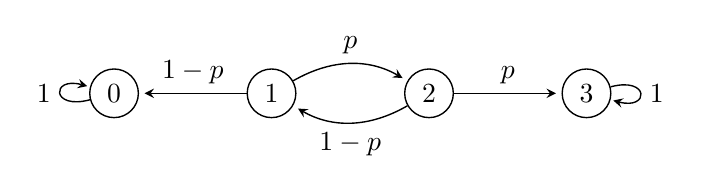
\begin{tikzpicture}[->,>=stealth,shorten >=2pt , line width=0.5 pt, node distance=2cm]

\node [circle, draw] (zero) {0};
\node [circle, draw] (one) [right of=zero] {1};
\node [circle, draw] (two) [ right of=one] {2};
\node [circle, draw] (three) [ right of=two] {3};
\path (zero) edge [loop left] node {$1$} (zero) ;
\path (one) edge node [above] {$1 - p$} (zero) ;
\path (one) edge [bend left] node [above]{$p$} (two) ;
\path (two) edge node [above]{$p$} (three) ;
\path (two) edge [bend left] node [below]{$1 - p$} (one) ;
\path (three) edge [loop right] node {$1$} (three) ;


\end{tikzpicture} \\
\end{center}
Above is an illustration of the Gambler's Ruin Problem.

\subsection{References}

The equation and its description were referenced from the following sources:
\begin{itemize}
    \item Wikipedia - Markov Chains \footnote{\url{https://en.wikipedia.org/wiki/Markov_chain}} 
    \item New York University - Lecture Handouts - Markov Chains \footnote{\url{https://cims.nyu.edu/~holmes/teaching/asa19/handout_Lecture2_2019.pdf}}
\end{itemize}



\end{document}
